%% ============================================================
%%  MEMORIA TECNICA - UNIDAD I: REDES DE COMUNICACION I
%%  Biblioteca "La Cantera" - Infraestructura Fisica y
%%  Cableado Estructurado (Capas 1 y 2 OSI)
%%  Compilar: pdflatex main.tex (ejecutar DOS veces para TOC)
%% ============================================================
\documentclass[12pt,a4paper]{article}

\usepackage[utf8]{inputenc}
\usepackage[T1]{fontenc}
\usepackage[spanish,es-tabla,es-nodecimaldot]{babel}
\usepackage{lmodern}
\usepackage{amssymb}
\usepackage{microtype}
\usepackage[top=2.5cm,bottom=2.5cm,left=3.0cm,right=2.5cm]{geometry}
\usepackage[dvipsnames,table]{xcolor}
\usepackage{graphicx}
\usepackage{float}
\usepackage{subcaption}
\usepackage{booktabs}
\usepackage{tabularx}
\usepackage{longtable}
\usepackage{array}
\usepackage{enumitem}
\usepackage{listings}
\usepackage{tcolorbox}
\tcbuselibrary{skins,breakable}
\usepackage{fancyhdr}
\usepackage{lastpage}
\usepackage{titlesec}
\usepackage[hidelinks]{hyperref}
\usepackage{parskip}
\usepackage{setspace}
\usepackage{fontawesome5}

%% ── Colores ─────────────────────────────────────────────────
\definecolor{azulUni}{RGB}{0,51,102}
\definecolor{azulClaro}{RGB}{0,102,179}
\definecolor{grisTabla}{RGB}{230,236,245}
\definecolor{verdeTech}{RGB}{0,120,80}
\definecolor{rojoCaution}{RGB}{180,30,30}
\definecolor{grisHeaders}{RGB}{44,62,80}

%% ── Cabecera y pie ──────────────────────────────────────────
\pagestyle{fancy}\fancyhf{}
\renewcommand{\headrulewidth}{1.5pt}
\renewcommand{\footrulewidth}{0.5pt}
\fancyhead[L]{\small\color{azulUni}\textbf{Redes de Comunicacion I -- Unidad I}}
\fancyhead[R]{\small\color{azulUni}Biblioteca ``La Cantera'' -- Cableado Estructurado}
\fancyfoot[C]{\small\color{gray}Memoria Tecnica de Ingenieria}
\fancyfoot[R]{\small\color{azulUni}\textbf{Pag.\ \thepage\ de \pageref{LastPage}}}

%% ── Secciones ───────────────────────────────────────────────
\titleformat{\section}{\Large\bfseries\color{azulUni}}
  {\color{azulClaro}\S\thesection}{0.8em}{}[\color{azulClaro}\titlerule]
\titleformat{\subsection}{\large\bfseries\color{azulClaro}}
  {\thesubsection}{0.7em}{}
\titleformat{\subsubsection}{\normalsize\bfseries\color{grisHeaders}}
  {\thesubsubsection}{0.6em}{}

%% ── Cajas ───────────────────────────────────────────────────
\newtcolorbox{cajanorma}[1]{colback=blue!5!white,colframe=azulUni,
  fonttitle=\bfseries\small\color{white},title={#1},arc=3mm,
  boxrule=1.2pt,left=6pt,right=6pt,breakable}
\newtcolorbox{cajawarning}{colback=yellow!10!white,colframe=rojoCaution,
  fonttitle=\bfseries\small\color{white},
  title={Nota de Exclusion del Diseno},arc=3mm,boxrule=1pt,left=6pt,right=6pt}
\newtcolorbox{cajatecnica}[1]{colback=green!5!white,colframe=verdeTech,
  fonttitle=\bfseries\small\color{white},title={#1},arc=3mm,
  boxrule=1pt,left=6pt,right=6pt,breakable}

%% ── Codigo CLI ──────────────────────────────────────────────
\lstset{language=bash,backgroundcolor=\color{black!90},
  basicstyle=\small\ttfamily\color{green!70!white},
  keywordstyle=\color{cyan},commentstyle=\color{gray},
  frame=single,framerule=0pt,breaklines=true,
  numbers=left,numberstyle=\tiny\color{gray},
  xleftmargin=1.5em,rulecolor=\color{black!60}}

\hypersetup{pdftitle={Memoria Tecnica -- LAN Biblioteca La Cantera},
  pdfauthor={Grupo Redes I -- 2026},
  pdfsubject={Cableado Estructurado Unidad I}}

\setstretch{1.15}

%% ============================================================
\begin{document}

%% ── PORTADA ─────────────────────────────────────────────────
\thispagestyle{empty}
\begin{titlepage}
  \noindent\colorbox{azulUni}{\parbox{\textwidth}{\vspace{0.6cm}\centering
    %% LOGOS: Descomentar y ajustar rutas cuando tengas los archivos:
    %% \includegraphics[height=2.5cm]{logo_universidad.png}\hspace{1.5cm}
    %% \includegraphics[height=2.5cm]{logo_facultad.png}
    %%
    %% Por ahora se muestran recuadros de referencia:
    \fbox{\parbox{3cm}{\centering\color{white}\footnotesize Logo\\Universidad\vspace{0.25cm}}}
    \hspace{1cm}
    \fbox{\parbox{3cm}{\centering\color{white}\footnotesize Logo\\Facultad\vspace{0.25cm}}}
    \vspace{0.5cm}}}

  \vspace{0.4cm}
  \begin{center}
    {\large\bfseries\color{azulUni}[NOMBRE DE LA UNIVERSIDAD]}\\[0.1cm]
    {\normalsize\color{azulClaro}Facultad de Ingenieria de Sistemas e Informatica}\\[0.05cm]
    {\small\color{gray}Escuela Profesional de Ingenieria de Sistemas / Computacion}
  \end{center}

  \vspace{0.4cm}
  \noindent\color{azulClaro}\rule{\textwidth}{1.5pt}\vspace{0.3cm}

  \begin{center}
    {\small\bfseries\color{grisHeaders}MEMORIA TECNICA DE INGENIERIA -- UNIDAD I}\\[0.5cm]
    {\LARGE\bfseries\color{azulUni}
      Diseno de la Infraestructura Fisica y\\[0.2cm]
      Cableado Estructurado de una Red LAN\\[0.3cm]}
    \noindent\color{azulClaro}\rule{0.6\textwidth}{0.8pt}\\[0.3cm]
    {\large\bfseries\color{verdeTech}Biblioteca ``La Cantera''}\\[0.2cm]
    {\normalsize\itshape\color{gray}
      Capas 1 (Fisica) y 2 (Enlace de Datos) del Modelo OSI}
  \end{center}

  \vspace{0.5cm}
  \noindent\color{azulClaro}\rule{\textwidth}{1.5pt}\vspace{0.6cm}

  \begin{center}
  \begin{tabular}{ll}
    \toprule
    \multicolumn{2}{c}{\bfseries\color{azulUni}Equipo de Trabajo -- Grupo N.\ {[\,]}} \\
    \midrule
    \bfseries Integrante 1: & [Apellidos y Nombres] \\
      & \small\itshape\color{gray}Analisis de la organizacion, problematica y requerimientos\\[3pt]
    \bfseries Integrante 2: & [Apellidos y Nombres] \\
      & \small\itshape\color{gray}Fundamentos, topologias, modelos OSI/TCP-IP y encapsulacion\\[3pt]
    \bfseries Integrante 3: & [Apellidos y Nombres] \\
      & \small\itshape\color{gray}Capa fisica, senales y seleccion de medios de transmision\\[3pt]
    \bfseries Integrante 4: & [Apellidos y Nombres] \\
      & \small\itshape\color{gray}Cableado estructurado, normas, rack y armado fisico UTP\\[3pt]
    \bfseries Integrante 5: & [Apellidos y Nombres] \\
      & \small\itshape\color{gray}Plano fisico, materiales, plan de pruebas y consolidacion\\[6pt]
    \bfseries Curso:    & Redes de Comunicacion I \\
    \bfseries Docente:  & [Nombre del Docente] \\
    \bfseries Ciclo:    & [Ciclo Academico] \\
    \bfseries Fecha:    & Octubre, 2026 \\
    \bottomrule
  \end{tabular}
  \end{center}

  \vfill
  \noindent\colorbox{azulUni}{\parbox{\textwidth}{\centering\vspace{0.3cm}
    {\small\color{white}
      \textbf{Curso:} Redes de Comunicacion I \quad|\quad
      \textbf{Unidad I} \quad|\quad \textbf{Anio:} 2026}
    \vspace{0.3cm}}}
\end{titlepage}

\thispagestyle{empty}
\tableofcontents
\clearpage

%% ============================================================
\section{Introduccion}

Las bibliotecas modernas han evolucionado de simples repositorios pasivos de libros a \textbf{Centros de Recursos para el Aprendizaje y la Investigacion (CRAI)}. El acceso instantaneo a catalogos en linea (OPAC), bases de datos cientificas, libros digitales y aulas virtuales constituye un servicio de primera necesidad para estudiantes y personal.

Para posibilitar esta interaccion digital, la infraestructura de telecomunicaciones fisica representa los cimientos indispensables. Una red LAN deficiente genera interrupciones constantes, frustracion en los usuarios y cuellos de botella en la administracion del patrimonio bibliografico.

El presente proyecto aborda el \textbf{diseno integral de la infraestructura fisica y el cableado estructurado} para la \textbf{Biblioteca ``La Cantera''}, entidad educativa de mediana escala. El diseno se fundamenta en la \textbf{Capa 1 (Fisica) y Capa 2 (Enlace)} del modelo OSI, conforme a las normativas internacionales \textbf{ANSI/TIA-568}, TIA-569 e ISO/IEC 11801, garantizando una solucion robusta, escalable y de alto rendimiento para 30 a 60 dispositivos simultaneos.

%% ============================================================
\section{Descripcion de la Organizacion}

\subsection{Actividad y Servicios}

\begin{itemize}[leftmargin=1.5em,itemsep=2pt]
  \item Prestamo y devolucion automatizada de material bibliografico fisico.
  \item Consulta del catalogo en linea (OPAC) y prestamo de libros electronicos.
  \item Zona de estudio silencioso individual e investigacion especializada.
  \item Modulos de estudio grupal con 6 laptops estudiantiles en 3 cubiculos.
  \item Sala de computo con 16 PCs conectadas a Internet de alta velocidad.
  \item Servicios de impresion en red y digitalizacion de documentos.
\end{itemize}

\subsection{Ambientes Fisicos y Distribucion Espacial}

El local comprende \textbf{500 m$^2$} (25 m $\times$ 20 m) con los siguientes ambientes:

\begin{enumerate}[leftmargin=1.8em,itemsep=3pt]
  \item \textbf{Recepcion, Prestamo y Circulacion:} 3 puestos de bibliotecarios.
  \item \textbf{Sala de Computo Estudiantil:} 16 PCs para investigacion academica.
  \item \textbf{Modulos OPAC (4 terminales):} Consulta rapida del catalogo en pasillos.
  \item \textbf{Sala de Lectura General:} Area abierta para estudiantes con laptops.
  \item \textbf{Cubiculos de Estudio Grupal (3 salas):} 2 laptops por cubiculo (6 total) via Wi-Fi al AP-03 (SSID: \texttt{Wifi-Cubiculos}).
  \item \textbf{Oficina de Direccion y Catalogacion:} 2 puestos para gestion bibliografica.
  \item \textbf{Cuarto de Telecomunicaciones (MDF):} Sala tecnica 2.5$\times$3.0 m, equidistante para que ningun tiro de cable supere los 90 m normativos.
\end{enumerate}

\subsection{Poblacion y Usuarios}

\begin{itemize}[leftmargin=1.5em,itemsep=2pt]
  \item \textbf{Personal Bibliotecario y Administrativo:} 6 personas permanentes.
  \item \textbf{Estudiantes e Investigadores Concurrentes:} Hasta 70 personas en horas pico.
\end{itemize}

%% ============================================================
\section{Problematica}

\begin{enumerate}[leftmargin=1.8em,label=\textbf{\arabic*.},itemsep=4pt]
  \item \textbf{Monopolio y saturacion de un unico AP domestico:} Con mas de 10--15 conexiones simultaneas se producen caidas de senal Wi-Fi y perdida de paquetes severa en los 500 m$^2$ del local.

  \item \textbf{Zonas muertas por estanterias metalicas:} Los libros y estanterias actuan como pantallas atenuadoras de RF en 2.4 GHz y 5 GHz. Los cubiculos y la sala de computo carecen practicamente de cobertura.

  \item \textbf{Inexistencia de puestos fijos cableados:} Los estudiantes dependen del Wi-Fi inestable. La sala de computo usaba mini-switches en cascada, causando navegacion extremadamente lenta.

  \item \textbf{Interferencia entre trafico administrativo y estudiantil:} Todo el trafico compite en el mismo medio fisico sin segmentacion de puertos.

  \item \textbf{Riesgo fisico por cableado desorganizado:} Cables tendidos por el zocalo o pasillos con cinta adhesiva representan peligro de tropiezo y dano mecanico al cable UTP.
\end{enumerate}

%% ============================================================
\section{Objetivos}

\subsection{Objetivo General}
Disenar y dimensionar tecnicamente la infraestructura fisica y el sistema de cableado estructurado de una red LAN para la Biblioteca ``La Cantera'', cumpliendo los estandares \textbf{ANSI/TIA-568}, TIA-569 e ISO/IEC 11801, asegurando conectividad Gigabit cableada y distribucion estrategica de 4 Access Points Wi-Fi 6.

\subsection{Objetivos Especificos}
\begin{enumerate}[leftmargin=1.8em,itemsep=3pt]
  \item Relevar y clasificar los requerimientos de conectividad para 30 a 60 nodos activos.
  \item Reemplazar el unico AP domestico mediante 4 Access Points empresariales Wi-Fi 6.
  \item Disenar el cableado horizontal Cat 6 para 16 PCs y 4 modulos OPAC.
  \item Centralizar las conexiones en un Rack 24U (MDF) con Switches Cisco Catalyst 2960.
  \item Elaborar la lista de materiales (BOM), detallando rosetas, canaletas y metrado UTP.
  \item Definir el plan de pruebas fisicas con LAN Tester para verificar continuidad y T568B.
\end{enumerate}

%% ============================================================
\section{Requerimientos de Red}

\subsection{Inventario de Dispositivos y Nodos de Conexion}

\rowcolors{2}{grisTabla}{white}
\begin{longtable}{>{\bfseries\small}p{2.8cm}>{\small}p{3.2cm}>{\small}p{2.2cm}>{\centering\small\bfseries}p{1.2cm}>{\small}p{3.6cm}}
  \toprule
  \rowcolor{azulUni}
  \color{white}Ambiente&\color{white}Dispositivo&\color{white}Conexion&\color{white}Cant.&\color{white}Descripcion Tecnica\\
  \midrule\endfirsthead
  \toprule
  \rowcolor{azulUni}
  \color{white}Ambiente&\color{white}Dispositivo&\color{white}Conexion&\color{white}Cant.&\color{white}Descripcion\\
  \midrule\endhead
  \bottomrule\endlastfoot
  Sala de Computo  & PCs Estudiantiles      & UTP Cat 6      & 16 & Investigacion academica. \\
  Pasillos / OPAC  & Terminales OPAC        & UTP Cat 6      & 4  & Busqueda rapida del catalogo. \\
  Cubiculos        & Laptops (via AP-03)    & Wi-Fi 6        & 6  & 2 laptops/cubiculo, inalambrico. \\
  Recepcion        & PCs Bibliotecarios     & UTP Cat 6      & 3  & Control de prestamos. \\
  Recepcion        & Impresora de Red       & UTP Cat 6      & 1  & Impresion de fichas. \\
  Direccion        & PCs Administrativas    & UTP Cat 6      & 2  & Catalogacion y gestion. \\
  MDF              & Servidor NAS Central   & UTP Cat 6 1Gbps& 1  & OPAC y repositorio. \\
  Techo            & Access Points Wi-Fi 6  & UTP Cat 6 PoE  & 4  & AP-01 a AP-04, cobertura sectorizada. \\
  Acceso Principal & Camara IP Domo         & UTP Cat 6      & 1  & Vigilancia; Ceiling Mount. \\
  \midrule
  \multicolumn{3}{r}{\bfseries TOTAL PUNTOS CABLEADOS}&
  \bfseries\color{azulUni}38&Distribuidos en 2 Patch Panels de 24 puertos.\\
\end{longtable}

\subsection{Capacidad de Access Points (Usuarios Inalambricos)}
\begin{itemize}[leftmargin=1.5em,itemsep=2pt]
  \item \textbf{AP-01} (Sala de Lectura): 30--40 conexiones simultaneas.
  \item \textbf{AP-02} (Sala de Computo): 20 dispositivos complementarios.
  \item \textbf{AP-03} (Cubiculos -- SSID \texttt{Wifi-Cubiculos}): 6 laptops fijas + moviles.
  \item \textbf{AP-04} (Recepcion): 15 conexiones de personal y usuarios en transito.
\end{itemize}

%% ============================================================
\section{Tipo y Topologia de Red}

\subsection{Clasificacion por Alcance: Red de Area Local (LAN)}
La infraestructura corresponde a una \textbf{LAN} por: ambito geografico limitado a 500 m$^2$, propiedad y control privado de la institucion, y tecnologia Gigabit Ethernet con velocidades de 1000 Mbps y latencias $<$1 ms.

\subsection{Topologia Fisica: Estrella Extendida -- Seccion 7}

La \textbf{Topologia en Estrella Extendida} esta centralizada en el MDF con dos Switches \textbf{Cisco Catalyst 2960-24TT} interconectados via \texttt{GigabitEthernet0/1} (troncal 1000 Mbps). El Router-WAN (Cisco 2911) se conecta al Switch-MDF-1 via \texttt{GigabitEthernet0/0} con IP 192.168.1.1/24.

\begin{figure}[H]
  \centering
  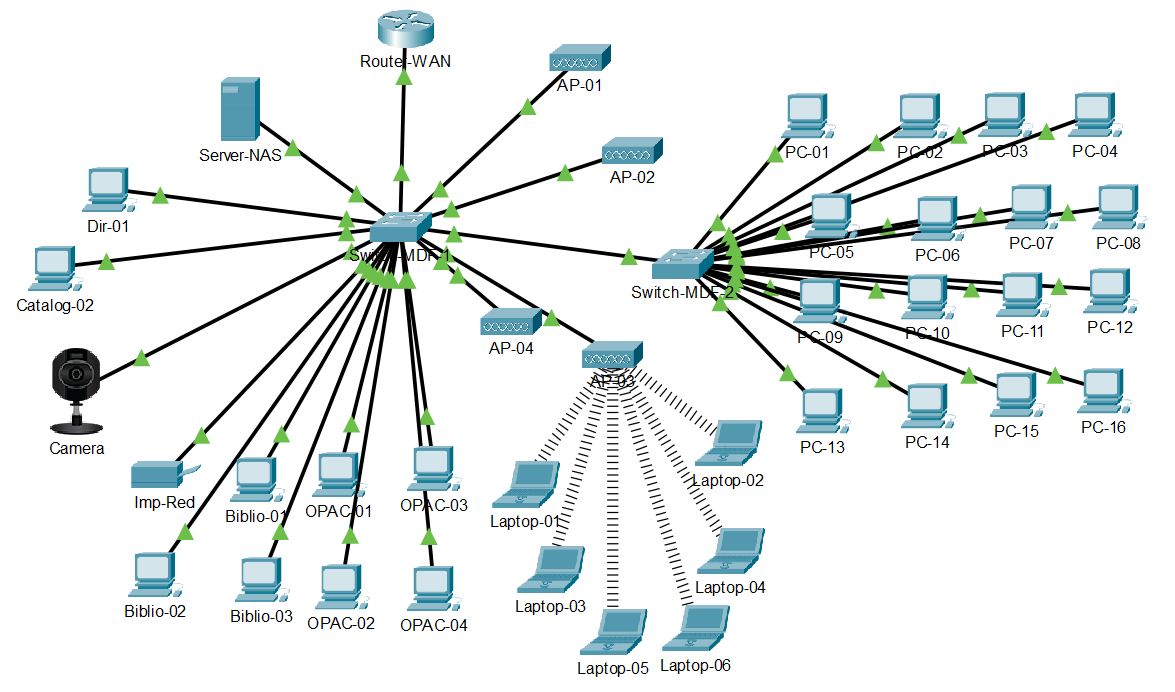
\includegraphics[width=0.88\textwidth]{topologia_logica.png}
  \caption{Topologia Logica -- Biblioteca ``La Cantera'' (Cisco Packet Tracer)}
  \label{fig:topologia}
\end{figure}

\subsubsection{Justificacion Tecnica: Estrella Extendida vs.\ Bus vs.\ Anillo}

\rowcolors{2}{grisTabla}{white}
\begin{tabularx}{\textwidth}{>{\bfseries\small}X>{\small}X>{\small}X>{\small\bfseries\color{verdeTech}}X}
  \toprule
  \rowcolor{azulUni}
  \color{white}Criterio&\color{white}Bus&\color{white}Anillo&\color{white}Estrella Extendida \checkmark\\
  \midrule
  Aislamiento de fallas & Un nodo cae, toda la red cae & Un nodo cae, toda la red cae & Un nodo cae, solo ese puerto \\
  Diagnostico & Sin punto central, muy dificil & Requiere recorrer el anillo & Inmediato en el Patch Panel \\
  Escalabilidad & Muy limitada (bus saturado) & Limitada, romper el anillo & Alta: agregar roseta sin interrumpir \\
  Norma ANSI/TIA-568 & Prohibida para horizontal & Prohibida para horizontal & Exigida y estandarizada \\
  Rendimiento & Half-Duplex, con colisiones & Dependiente de token & Full-Duplex, sin colisiones \\
  \bottomrule
\end{tabularx}
\vspace{6pt}

\begin{cajanorma}{Conclusion -- Justificacion de la Topologia en Estrella Extendida}
La norma \textbf{ANSI/TIA-568} prohibe taxativamente las topologias de bus o anillo para cableado horizontal comercial, exigiendo que cada toma de telecomunicaciones este conectada directamente a un distribuidor central en estrella punto a punto. La Estrella Extendida satisface esta exigencia ofreciendo \textbf{aislamiento total de fallas}, diagnostico inmediato desde el MDF y plena escalabilidad sin interrupcion del servicio.
\end{cajanorma}

\subsection{Topologia Logica}
\begin{itemize}[leftmargin=1.5em,itemsep=3pt]
  \item \textbf{Dominio Cableado (IEEE 802.3):} Full-Duplex conmutado; cada puerto del Cisco 2960 es un dominio de colision independiente. No existen colisiones en los cables UTP Cat 6.
  \item \textbf{Dominio Inalambrico (IEEE 802.11ax / Wi-Fi 6):} Medio compartido por \textbf{CSMA/CA}. AP-03 opera con SSID exclusivo \texttt{Wifi-Cubiculos} para las 6 laptops estudiantiles.
\end{itemize}

%% ============================================================
\section{Modelos de Referencia: OSI y TCP/IP}

\subsection{Mapeo de Capas en el Contexto de la Biblioteca}

\rowcolors{2}{grisTabla}{white}
\begin{tabularx}{\textwidth}{>{\centering\bfseries\small}p{1.4cm}>{\small}p{2cm}>{\small}p{1.8cm}>{\small}p{3.1cm}>{\small}X}
  \toprule
  \rowcolor{azulUni}
  \color{white}Capa OSI&\color{white}Funcion&\color{white}TCP/IP&\color{white}Elementos en Biblioteca&\color{white}Protocolos\\
  \midrule
  7. Aplicacion & Interfaz usuario y servicios & \multirow{3}{*}{Aplicacion} & Catalogo OPAC, navegador web & HTTP, HTTPS, DNS, DHCP \\
  6. Presentacion & Formato y cifrado & & Cifrado de credenciales & TLS 1.3, HTML5 \\
  5. Sesion & Control del dialogo & & Sesion del estudiante & SSL/TLS, RPC \\
  4. Transporte & Entrega confiable & Transporte & Segmentacion de descargas & TCP (443), UDP (53) \\
  3. Red & Enrutamiento logico & Internet & Router-WAN de borde & IPv4, ICMP, ARP \\
  2. Enlace & Direccionamiento MAC, trama & \multirow{2}{*}{Acceso Red} & Switches Cisco 2960, NICs PCs & IEEE 802.3, 802.11 \\
  \rowcolor{green!12}\textbf{1. Fisica} & \textbf{Transmision de bits} & & \textbf{UTP Cat 6, RJ-45, Jacks, Patch Panels, ondas RF} & \textbf{PAM-5, 1000BASE-T} \\
  \bottomrule
\end{tabularx}
\begin{center}\small\itshape
El proyecto se enfoca en las Capas 1 y 2 (resaltadas), conforme a la rubrica de evaluacion.
\end{center}

\subsection{Proceso de Encapsulacion y Desencapsulacion}
\textbf{Escenario:} Un estudiante en la Sala de Computo (PC cableada UTP Cat 6) busca el libro \textit{``Redes de Computadoras'' de Tanenbaum} en el catalogo OPAC.

\begin{enumerate}[leftmargin=1.8em,itemsep=3pt]
  \item \textbf{Aplicacion (7):} El navegador envia \texttt{GET /catalogo?libro=tanenbaum HTTP/1.1}.
  \item \textbf{Transporte (4):} Se agrega cabecera TCP (puerto efimero origen; destino 80/443). Se genera el \textit{Segmento}.
  \item \textbf{Red (3):} Se incorpora encabezado IP (IP-origen: PC; IP-destino: Servidor NAS). Se genera el \textit{Paquete}.
  \item \textbf{Enlace (2):} La NIC agrega la \textbf{Trama Ethernet 802.3} con MAC-origen, MAC-destino y \textbf{FCS/CRC-32} al final. Se genera la \textit{Trama}.
  \item \textbf{Fisica (1):} La NIC convierte los bits en pulsos electricos via modulacion \textbf{PAM-5}. Las senales viajan por los 4 pares del UTP Cat 6 a traves del Jack Keystone, la canaleta PVC, el Patch Panel, los Switches Cisco 2960 y llegan al Servidor NAS.
\end{enumerate}

%% ============================================================
\section{Sistemas y Medios de Comunicacion (Capa Fisica)}

\subsection{Tipos de Senales en la Biblioteca}
\begin{itemize}[leftmargin=1.5em,itemsep=3pt]
  \item \textbf{Senales Electricas Conducidas (UTP Cat 6):} Informacion binaria como variaciones de voltaje sobre cobre balanceado. El estandar \textbf{1000BASE-T} usa modulacion \textbf{PAM-5} a 125 MBaudios por par en los 4 pares simultaneamente (Full-Duplex).
  \item \textbf{Senales Electromagneticas (Wi-Fi 6 / IEEE 802.11ax):} Ondas de radio en 2.4 GHz y 5 GHz mediante \textbf{1024-QAM} y division de frecuencias ortogonales (\textbf{OFDMA}).
\end{itemize}

\subsection{Factores de Degradacion y Mitigacion}
\begin{enumerate}[leftmargin=1.8em,label=\textbf{\arabic*.},itemsep=4pt]
  \item \textbf{Atenuacion:} Perdida progresiva de potencia. La norma ANSI/TIA-568 establece un limite de \textbf{90 m de enlace permanente}. El punto mas lejano del proyecto (AP-01) se ubica a solo \textbf{38 m}, con mas del 57\% de margen de seguridad.

  \item \textbf{Ruido EMI/RFI:} Causado por balastros de lamparas y cableado de 220 VAC. \textit{Mitigacion:} Separacion minima de \textbf{20--30 cm} entre canaletas de datos y conductores electricos; cruce en angulo recto (90$^\circ$).

  \item \textbf{Diafonia (Crosstalk / NEXT):} Interferencia inductiva entre pares adyacentes. Cat 6 incorpora una \textbf{cruceta plastica interna (spline)} que separa fisicamente los cuatro pares, reduciendo el NEXT drasticamente.

  \item \textbf{Atenuacion RF en Cubiculos:} Las estanterias metalicas absorben y dispersan la senal. \textit{Mitigacion:} 4 APs con linea de vista directa en cada zona funcional, eliminando zonas muertas.
\end{enumerate}

%% ============================================================
\section{Seleccion y Justificacion de Medios de Transmision}

\begin{cajanorma}{Seccion 10 -- Tabla Comparativa de Medios de Transmision para Cableado Horizontal}
Analisis tecnico y economico de los tres principales candidatos de medio fisico para el proyecto de la Biblioteca ``La Cantera''.
\end{cajanorma}

\rowcolors{2}{grisTabla}{white}
\begin{tabularx}{\textwidth}{>{\bfseries\small}p{3cm}>{\small}X>{\small}X>{\small\bfseries\color{verdeTech}}X}
  \toprule
  \rowcolor{azulUni}
  \color{white}Criterio&\color{white}Coaxial (RG-6/RG-58)&\color{white}Fibra Optica (OM3/OM4)&\color{white}UTP Cat 6 \checkmark\\
  \midrule
  Ancho de Banda    & Bajo: 10--100 MHz, obsoleto & Extremadamente alto: $>$10 GHz & \textbf{Alto: 250 MHz / 1--10 Gbps} \\
  Distancia Maxima  & 185--500 m & 300 m (multi) a 40 km (mono) & \textbf{100 m total; 90 m enlace perm.} \\
  Costo por punto   & Bajo--medio, obsoleto en LAN & Alto (transceivers, fusiones) & \textbf{Muy economico, alta disponibilidad} \\
  Inmunidad al ruido & Moderada (malla metalica) & Total (fotones, 100\% inmune) & \textbf{Alta con Cat 6 y separacion 220 V} \\
  Conectorizado     & Engorroso en masa & Muy complejo (fusionadora) & \textbf{Rapido: crimpado RJ-45 y punch-down} \\
  Soporte PoE       & Nulo & Nulo (no conduce electricidad) & \textbf{Excelente: IEEE 802.3at hasta 30 W} \\
  \textbf{Veredicto}& \color{rojoCaution}Descartado (obsoleto) & \color{rojoCaution}Descartado (sobrecosto $<$40 m) & \color{verdeTech}\textbf{SELECCIONADO} \\
  \bottomrule
\end{tabularx}
\vspace{6pt}

\textbf{Justificacion clave de UTP Cat 6:}
\begin{enumerate}[leftmargin=1.8em,itemsep=3pt]
  \item \textbf{Rendimiento garantizado:} 38 m de distancia maxima frente al limite de 90 m. Cat 6 entrega 1 Gbps a 250 MHz con amplio margen de atenuacion.
  \item \textbf{PoE nativo:} Los 4 APs y la camara IP se alimentan por el mismo cable (IEEE 802.3at), eliminando el cableado electrico de 220 V en el falso techo.
  \item \textbf{Conductor 100\% Cobre Solido 23 AWG:} Se prohibe el cable CCA (Copper Clad Aluminum), que presenta alta resistencia ohmica y se quiebra en canaletas.
  \item \textbf{Costo-beneficio:} La fibra queda reservada unicamente para la acometida del ISP hacia el Router-WAN.
\end{enumerate}

%% ============================================================
\section{Cableado Estructurado}

\begin{cajanorma}{Seccion 11 -- Marco Normativo Internacional Aplicable}
  \begin{itemize}[leftmargin=1em,itemsep=2pt]
    \item \textbf{ANSI/TIA-568-C / ANSI/TIA-568.2-D:} Estandar de cableado para edificios comerciales -- Categoria 6.
    \item \textbf{ANSI/TIA-569-D:} Estandar de espacios y canalizaciones de telecomunicaciones.
    \item \textbf{ANSI/TIA-606-B:} Estandar de administracion y etiquetado de la infraestructura.
    \item \textbf{ISO/IEC 11801:} Estandar internacional generico de cableado para instalaciones de clientes.
  \end{itemize}
\end{cajanorma}

\subsection{Subsistemas de Cableado Implementados}
\begin{enumerate}[leftmargin=1.8em,label=\textbf{\arabic*.},itemsep=3pt]
  \item \textbf{Acometida (ISP):} Llega desde la via publica hacia el MDF.
  \item \textbf{Cuarto de Telecomunicaciones (MDF):} Rack 24U con Patch Panels, Switches Cisco 2960, Router 2911 y Servidor NAS.
  \item \textbf{Cableado Horizontal:} UTP Cat 6 solido 23 AWG en canaletas PVC, desde el MDF hasta cada area de trabajo. Distancia maxima real: \textbf{38 m} (limite normativo: 90 m).
  \item \textbf{Area de Trabajo:} 7 Copper Wall Mounts (rosetas doble puerto) y 1 Ceiling Mount para la camara IP.
\end{enumerate}

\subsubsection{Regla de Distancias del Canal Horizontal (ANSI/TIA-568)}
\begin{itemize}[leftmargin=1.5em,itemsep=2pt]
  \item \textbf{Enlace Permanente:} Max.\ \textbf{90 m} (cable solido: Patch Panel $\to$ Jack Keystone).
  \item \textbf{Cables de Parcheo:} Max.\ \textbf{10 m} total (5 m en rack + 5 m en area de trabajo).
  \item \textbf{Canal Total:} Max.\ \textbf{100 m}.
  \item \textbf{Cumplimiento:} Distancia maxima en la biblioteca = 38 m. Margen de seguridad: $>$57\%.
\end{itemize}

\subsection{Norma T568B -- Codigo de Colores Adoptado (Segmentacion de Patch Panels)}

Se adopta \textbf{T568B de extremo a extremo} en la totalidad de la instalacion. La segmentacion en dos Patch Panels permite: (1) identificar rapidamente el trafico por origen (administrativo vs.\ estudiantil) y (2) facilitar el diagnosti co de fallas en el MDF sin confundir los cables.

\rowcolors{2}{grisTabla}{white}
\begin{tabularx}{\textwidth}{>{\centering\bfseries\small}p{0.9cm}>{\small}X>{\small\bfseries\color{verdeTech}}X>{\small}X}
  \toprule
  \rowcolor{azulUni}
  \color{white}Pin&\color{white}T568A&\color{white}T568B (Seleccionado)&\color{white}Funcion 1000BASE-T\\
  \midrule
  1 & Blanco/Verde   & \textbf{Blanco/Naranja} & Par Bi-dir A+ \\
  2 & Verde          & \textbf{Naranja}         & Par Bi-dir A- \\
  3 & Blanco/Naranja & \textbf{Blanco/Verde}    & Par Bi-dir B+ \\
  4 & Azul           & \textbf{Azul}            & Par Bi-dir C+ \\
  5 & Blanco/Azul    & \textbf{Blanco/Azul}     & Par Bi-dir C- \\
  6 & Naranja        & \textbf{Verde}           & Par Bi-dir B- \\
  7 & Blanco/Marron  & \textbf{Blanco/Marron}   & Par Bi-dir D+ \\
  8 & Marron         & \textbf{Marron}          & Par Bi-dir D- \\
  \bottomrule
\end{tabularx}
\vspace{6pt}

\textbf{Segmentacion de los dos Patch Panels -- importancia:}
\begin{itemize}[leftmargin=1.5em,itemsep=2pt]
  \item \textbf{Patch Panel 1 (U4--U5):} Dedicado a infraestructura troncal, gestion y Wi-Fi (AP-01 a AP-04, Router, Camara, Biblio, Dir, OPAC). Conectado exclusivamente al Switch-MDF-1.
  \item \textbf{Patch Panel 2 (U10--U11):} Dedicado en exclusiva al cableado horizontal de alta densidad de los 16 puestos estudiantiles. Conectado exclusivamente al Switch-MDF-2.
  \item Esta segmentacion garantiza \textbf{aislamiento de trafico}, \textbf{trazabilidad inmediata} de cada punto y \textbf{escalabilidad independiente} de ambos dominios.
\end{itemize}

\subsection{Distribucion del Rack de Telecomunicaciones (MDF -- 24U)}

\vspace{6pt}
\begin{center}
\rowcolors{1}{white}{grisTabla}
\begin{tabularx}{0.82\textwidth}{>{\centering\bfseries\small}p{1.6cm}>{\small}X}
  \toprule
  \rowcolor{azulUni}
  \color{white}Posicion (U)&\color{white}Elemento\\
  \midrule
  U4--U5   & Copper Patch Panel 1 -- 24 puertos Cat 6 (troncal, gestion y Wi-Fi; conectado a Switch-MDF-1) \\
  U7--U8   & \textbf{Switch Principal 1} -- Cisco Catalyst 2960-24TT (Switch-MDF-1) \\
  U10--U11 & Copper Patch Panel 2 -- 24 puertos Cat 6 (cableado horizontal estudiantil; conectado a Switch-MDF-2) \\
  U13--U14 & \textbf{Switch Principal 2} -- Cisco Catalyst 2960-24TT (Switch-MDF-2) \\
  U16--U18 & Router-WAN (Cisco 2911) + Servidor NAS de almacenamiento bibliografico \\
  \bottomrule
\end{tabularx}
\end{center}
\vspace{6pt}

\begin{figure}[H]
  \centering
  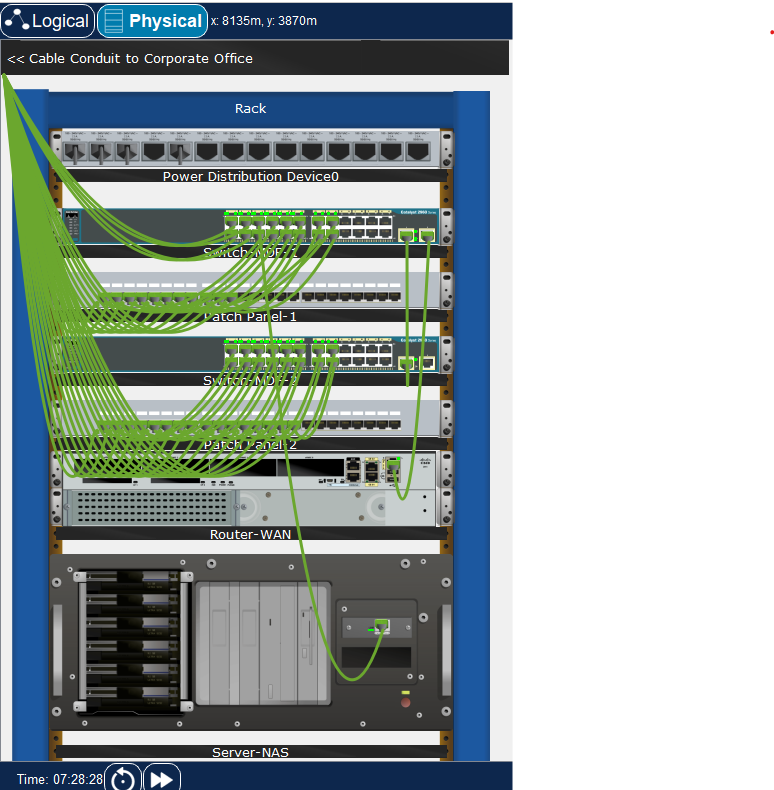
\includegraphics[width=0.54\textwidth]{main_wiring_closet.png}
  \caption{Vista Fisica del Rack MDF (24U) -- Cisco Packet Tracer (Physical View)}
  \label{fig:rack}
\end{figure}

\begin{cajawarning}
Se descartan en esta fase del proyecto las unidades \textbf{PDU/UPS} y sistemas de respaldo electrico por motivos de presupuesto inicial. Asimismo, se descartan las Smart TVs interactivas, priorizando cobertura Wi-Fi mediante AP-03 con SSID \texttt{Wifi-Cubiculos} para las laptops estudiantiles.
\end{cajawarning}

\subsection{Configuracion CLI del Router-WAN (Cisco 2911)}

\begin{lstlisting}[language=bash, caption={Configuracion CLI -- Interfaz GigabitEthernet0/0 del Router-WAN (Cisco 2911)}, label={lst:cli}]
Router> enable
Router# configure terminal
Router(config)# interface GigabitEthernet0/0
Router(config-if)# ip address 192.168.1.1 255.255.255.0
Router(config-if)# description Enlace-a-Switch-MDF-1
Router(config-if)# no shutdown
Router(config-if)# exit
Router(config)# end
Router# write memory
\end{lstlisting}

El enlace troncal entre ambos Switches usa las interfaces \texttt{GigabitEthernet0/1} de cada Cisco 2960, formando el backbone de alta velocidad de \textbf{1000 Mbps}.

%% ============================================================
\section{Diseno Fisico y Plano de Red}

\subsection{Plano General de la Biblioteca (Cisco Packet Tracer)}

\begin{figure}[H]
  \centering
  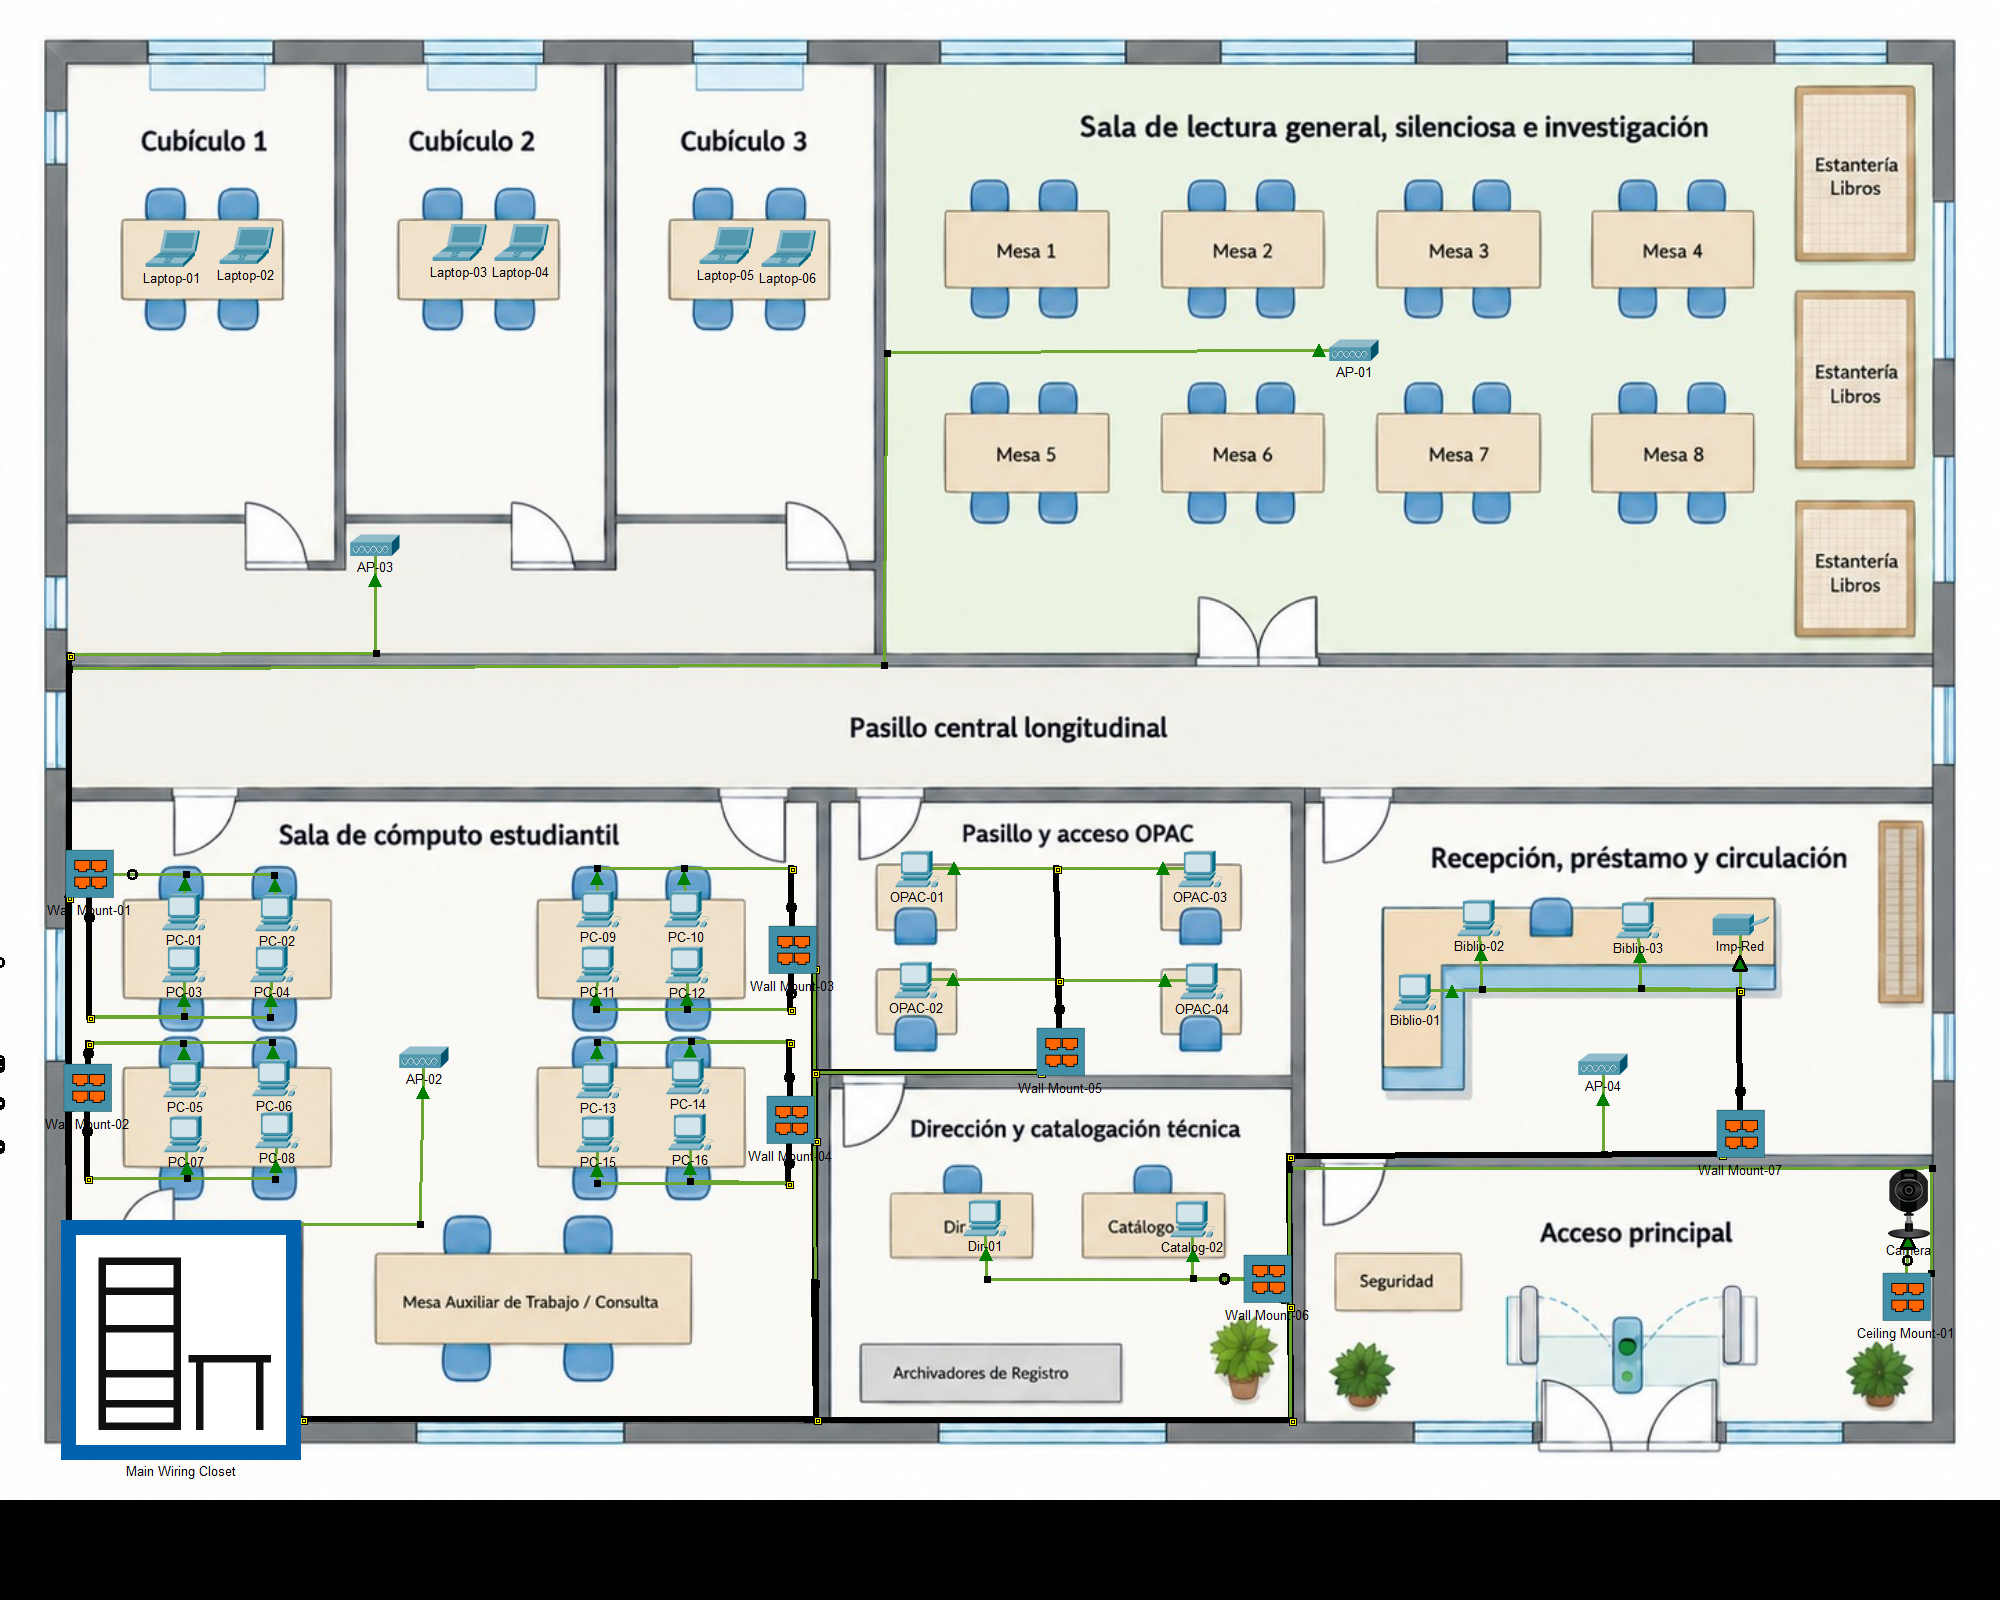
\includegraphics[width=\textwidth]{plano_pkt.png}
  \caption{Plano Fisico de la Red -- Biblioteca ``La Cantera'' (Cisco Packet Tracer -- Physical View)}
  \label{fig:plano}
\end{figure}

\subsection{Puntos de Acceso y Rosetas de Pared}
\begin{itemize}[leftmargin=1.5em,itemsep=3pt]
  \item \textbf{7 Copper Wall Mounts (rosetas doble puerto):} Wall-01 a Wall-04 (Sala Computo), Wall-05 (Pasillo OPAC), Wall-06 (Direccion/Catalogo), Wall-07 (Recepcion). Flujo normativo: \textbf{PC $\to$ Jack frontal $\to$ Punch-down trasero (cuchillas) $\to$ Canaleta PVC $\to$ Patch Panel}.
  \item \textbf{1 Ceiling Mount:} Acceso Principal para la Camara IP Domo de Seguridad; proporciona inmunidad mecanica y linea de vista total.
  \item \textbf{4 Access Points Wi-Fi 6 (AP-01 a AP-04):} Cableados al Switch-MDF-1 via PoE. AP-03 opera con SSID \texttt{Wifi-Cubiculos}.
\end{itemize}

\subsection{Rutas de Canalizacion}
\begin{itemize}[leftmargin=1.5em,itemsep=2pt]
  \item \textbf{Canaleta Principal (troncal):} PVC rigido 100$\times$50 mm con tabique interno para separar datos y alimentacion electrica.
  \item \textbf{Derivaciones secundarias:} PVC 40$\times$25 mm hacia cada puesto individual.
  \item \textbf{Falso techo:} Tubos conduit corrugados flexibles para la bajada a APs y Camara IP.
  \item \textbf{Bend Points:} Los cables se peinan por el contorno de los pasillos para evitar atenuacion y diafonia.
\end{itemize}

%% ============================================================
\section{Lista de Equipos y Materiales (BOM)}

\begin{cajanorma}{Seccion 13 -- Tabla Consolidada de Materiales (Sin PDU, UPS ni Smart TVs)}
BOM (\textit{Bill of Materials}) que contempla unicamente componentes de Capas Fisica y de Enlace, conforme a las exclusiones de presupuesto del diseno actual.
\end{cajanorma}

\rowcolors{2}{grisTabla}{white}
\begin{longtable}{>{\centering\bfseries\small}p{0.5cm}>{\small}p{1.9cm}>{\small}p{4.8cm}>{\centering\small}p{1.1cm}>{\centering\small}p{1cm}>{\small}p{3.6cm}}
  \toprule
  \rowcolor{azulUni}
  \color{white}\#&\color{white}Categoria&\color{white}Descripcion / Modelo Sugerido&\color{white}Cant.&\color{white}Unid.&\color{white}Justificacion\\
  \midrule\endfirsthead
  \toprule\rowcolor{azulUni}
  \color{white}\#&\color{white}Categoria&\color{white}Descripcion&\color{white}Cant.&\color{white}Unid.&\color{white}Justificacion\\
  \midrule\endhead\bottomrule\endlastfoot
  1  & Cable Pasivo   & Bobina UTP Cat 6, 100\% Cobre Solido, 23 AWG, LSZH (305 m/caja) & 2  & Cajas  & $\approx$550 m totales para todos los puntos de red \\
  2  & Switch Activo  & Cisco Catalyst 2960-24TT (24 puertos + 2 GbE uplink)             & 2  & Unid.  & Switch-MDF-1 y Switch-MDF-2; nucleo de conmutacion \\
  3  & Router         & Cisco 2911 -- Router-WAN de borde                                & 1  & Unid.  & Enlace WAN; IP de gestion 192.168.1.1/24 \\
  4  & Patch Panel    & Copper Patch Panel Cat 6, 24 puertos, 19'', 1U, IDC-110          & 2  & Unid.  & Remate ordenado del cableado horizontal en MDF \\
  5  & Rack           & Gabinete de piso metalico 19'', 24U, puerta vidrio templado       & 1  & Unid.  & Aloja todo el equipamiento activo y pasivo \\
  6  & Servidor NAS   & Servidor NAS de almacenamiento bibliografico con interfaz GbE     & 1  & Unid.  & Base de datos OPAC y repositorio institucional \\
  7  & Wi-Fi          & Access Point Empresarial Wi-Fi 6 (IEEE 802.11ax, Dual Band)       & 4  & Unid.  & Cobertura sectorizada AP-01 a AP-04 \\
  8  & Camara IP      & Camara IP Domo de Seguridad -- montaje Ceiling Mount              & 1  & Unid.  & Vigilancia del Acceso Principal \\
  9  & Jack Keystone  & Jack Hembra Cat 6 RJ-45, contactos 50 um oro                      & 20 & Unid.  & 7 Wall Mounts dobles (14 jacks) + Ceiling + repuestos \\
  10 & Wall Mount     & Copper Wall Mount -- roseta doble puerto (2 jacks keystone)       & 7  & Unid.  & PCs, Bibliotecarios, OPAC, Direccion, Recepcion \\
  11 & Ceiling Mount  & Ceiling Mount -- roseta para montaje en techo/muro alto           & 1  & Unid.  & Camara IP Domo de Seguridad \\
  12 & Conector RJ-45 & Conector Macho Cat 6 con guia de insercion y capuchon             & 50 & Unid.  & Armado de Patch Cords de prueba y terminales APs \\
  13 & Patch Cord     & Patch Cord Cat 6 moldeado de fabrica, 1.5 m, azul                & 30 & Unid.  & Conexion Patch Panel $\leftrightarrow$ Switch en Rack \\
  14 & Patch Cord     & Patch Cord Cat 6 moldeado de fabrica, 2.0 m, gris                & 20 & Unid.  & Conexion Faceplate $\leftrightarrow$ PC / dispositivo final \\
  15 & Canaleta       & Canaleta PVC rigido 100$\times$50 mm con tabique, tramos de 2 m  & 30 & Tramos & Troncal principal de distribucion por pasillos \\
  16 & Canaleta       & Canaleta PVC rigido 40$\times$25 mm, tramos de 2 m               & 40 & Tramos & Derivaciones secundarias a puestos individuales \\
  17 & Organizador    & Organizador horizontal de cables 19'', 1U, tapa desmontable       & 2  & Unid.  & Peinado de Patch Cords entre Patch Panel y Switch \\
  18 & Ponchadora     & Herramienta Punch-Down IDC-110 de impacto                         & 1  & Unid.  & Terminacion de jacks keystone y Patch Panels \\
\end{longtable}

%% ============================================================
\section{Plan de Pruebas y Certificacion de Cableado}

\begin{cajanorma}{Seccion 14 -- Plan de Pruebas Fisicas con LAN Tester (Herramienta de Certificacion)}
El siguiente plan valida la correcta operatividad fisica de la red antes de la puesta en produccion. Se utiliza el \textbf{LAN Tester RJ-45 (Master + Remote)} como herramienta principal de certificacion de la Capa Fisica.
\end{cajanorma}

\subsection{Prueba 1: Inspeccion Visual Mecanica (TIA-568.2-D)}
\begin{itemize}[leftmargin=1.5em,itemsep=2pt]
  \item Verificar que no existan mas de \textbf{13 mm} de cable destrenzado en conectores RJ-45 o jacks keystone.
  \item Confirmar que la chaqueta exterior ingrese al conector y quede fijada bajo la pestana de alivio de esfuerzo.
  \item Comprobar radios de curvatura no menores a \textbf{4 veces el diametro del cable} (min.\ 25 mm) para evitar microfracturas.
\end{itemize}

\subsection{Prueba 2: Continuidad y Mapa de Hilos (Wiremap Test)}
\begin{enumerate}[leftmargin=1.8em,itemsep=3pt]
  \item Conectar un extremo al \textbf{modulo Master} del LAN Tester y el otro al \textbf{modulo Remote}.
  \item \textbf{Criterio de aceptacion:} LEDs 1 al 8 se encienden secuencial y correlativamente en ambos modulos (1-1, 2-2, \ldots, 8-8).
\end{enumerate}

\textbf{Tabla de deteccion de defectos con LAN Tester:}

\rowcolors{2}{grisTabla}{white}
\begin{tabularx}{\textwidth}{>{\bfseries\small}p{3cm}>{\small}p{4cm}>{\small}X}
  \toprule
  \rowcolor{azulUni}
  \color{white}Defecto&\color{white}Indicacion en LAN Tester&\color{white}Causa Probable\\
  \midrule
  Circuito Abierto  & LED de un pin no enciende                      & Pin sin contacto; crimpado incompleto \\
  Cortocircuito     & Multiples LEDs encienden simultane             & Dos o mas conductores en contacto \\
  Par Cruzado       & LEDs invertidos (ej.: 1 y 2 cruzados)          & Extremos con orden diferente de hilos \\
  Par Dividido      & Continuidad pin a pin pero falla en link activo & Mezcla de pares; cancela el trenzado \\
  \bottomrule
\end{tabularx}

\subsection{Prueba 3: Enlace Activo y Autonegociacion (Link Speed Test)}
\begin{enumerate}[leftmargin=1.8em,itemsep=3pt]
  \item Conectar una laptop con NIC Gigabit a la roseta y el otro extremo al Switch Cisco 2960.
  \item Verificar LED del puerto del switch: \textbf{1000 Mbps Full-Duplex} (LED ambar o verde segun modelo).
  \item Ejecutar: \texttt{ping -t -l 1472 192.168.1.1} y verificar \textbf{0\% de perdidas de paquetes ICMP}.
\end{enumerate}

\subsection{Resumen del Plan de Pruebas}

\rowcolors{2}{grisTabla}{white}
\begin{tabularx}{\textwidth}{>{\bfseries\small}p{2.3cm}>{\small}p{2.8cm}>{\small}p{3cm}>{\small}X}
  \toprule
  \rowcolor{azulUni}
  \color{white}Prueba&\color{white}Herramienta&\color{white}Criterio de Aceptacion&\color{white}Accion ante Falla\\
  \midrule
  Inspeccion Visual & Observacion directa & 0 conductores expuestos; $<$13 mm destrenzados & Recrimpar o reemplazar el conector \\
  Wiremap           & LAN Tester RJ-45    & 8 LEDs secuenciales: 1-1 a 8-8 & Recrimpar el extremo defectuoso \\
  Link Speed        & NIC + Switch Cisco  & 1000 Mbps Full-Duplex (LED ambar/verde) & Verificar par dividido con Wiremap \\
  Perdida Paquetes  & \texttt{ping} extendido & 0\% perdidas; latencia $<$1 ms & Verificar distancia y calidad del cable \\
  \bottomrule
\end{tabularx}

%% ============================================================
\section{Conclusiones}

\begin{enumerate}[leftmargin=1.8em,label=\textbf{\arabic*.},itemsep=5pt]
  \item \textbf{Resolucion integral de la problematica:} El reemplazo del unico AP domestico por 4 Access Points Wi-Fi 6 distribuidos y 16 puestos fijos Gigabit Ethernet soluciona de raiz los cuellos de botella, la saturacion por alta concurrencia y las zonas muertas causadas por las estanterias metalicas.

  \item \textbf{Cumplimiento riguroso de ANSI/TIA-568:} La longitud maxima del recorrido es de 38 m, respetando el limite de 90 m del enlace permanente con mas del 57\% de margen de seguridad, garantizando transmision Gigabit a 250 MHz.

  \item \textbf{Estandarizacion T568B homogenea:} La adopcion uniforme de T568B en todos los componentes garantiza consistencia tecnica, reduce el tiempo de diagnostico y asegura compatibilidad con cualquier tecnico calificado.

  \item \textbf{Eficiencia economica mediante PoE:} La alimentacion de APs y camara IP a traves del cable de datos (IEEE 802.3at) elimino el cableado electrico de 220 V en el falso techo, reduciendo costos y elevando la seguridad contra incendios.

  \item \textbf{Escalabilidad de la Estrella Extendida:} Los dos Switches Cisco 2960 en cascada permiten incorporar nuevos dispositivos sin interrumpir el servicio, con puertos disponibles para expansiones futuras.
\end{enumerate}

%% ============================================================
\section{Referencias Bibliograficas}

\begin{enumerate}[leftmargin=1.8em,itemsep=4pt,label={[\arabic*]}]
  \item Telecommunications Industry Association. (2018). \textit{Balanced Twisted-Pair Telecommunications Cabling and Components Standard} (ANSI/TIA-568.2-D). TIA Standards.

  \item Telecommunications Industry Association. (2015). \textit{Telecommunications Pathways and Spaces} (ANSI/TIA-569-D). TIA Standards.

  \item International Organization for Standardization. (2017). \textit{Information technology -- Generic cabling for customer premises} (ISO/IEC 11801-1:2017). ISO.

  \item Kurose, J. F., \& Ross, K. W. (2021). \textit{Computer Networking: A Top-Down Approach} (8th ed.). Pearson.

  \item Tanenbaum, A. S., Feamster, N., \& Wetherall, D. (2021). \textit{Computer Networks} (6th ed.). Pearson.

  \item Stallings, W. (2017). \textit{Data and Computer Communications} (10th ed.). Pearson.

  \item Cisco Systems. (2023). \textit{Cisco Catalyst 2960-24TT Switch Datasheet}. Cisco Press. Recuperado de \url{https://www.cisco.com}

  \item IEEE. (2018). \textit{IEEE Standard for Ethernet} (IEEE Std 802.3-2018). IEEE.
\end{enumerate}

%% ============================================================
\section{Anexos}

\subsection{Anexo A: Factor de Llenado de Canaletas (TIA-569)}
El porcentaje de ocupacion inicial de las canaletas principales no excede el \textbf{40\%} de su capacidad transversal, dejando un 60\% de holgura para futuras expansiones sin comprometer la ventilacion ni ejercer presion mecanica sobre el cable UTP.

\subsection{Anexo B: Guia de Armado del Cable UTP (Para Evaluacion Practica)}

\begin{cajatecnica}{Procedimiento de Crimpado T568B -- Paso a Paso (Para defender en la exposicion)}
  \textbf{Materiales:} Cable UTP Cat 6 (1.5--2 m), 2 conectores macho RJ-45 Cat 6, capuchones, tenaza crimpadora 8P8C, pelacables, LAN Tester.
  \begin{enumerate}[leftmargin=1.5em,itemsep=2pt,label=\textbf{Paso \arabic*:}]
    \item Colocar capuchones protectores en ambos extremos \textit{antes} de crimpar.
    \item Pelar $\approx$2.5--3 cm de cubierta exterior sin mellar el cobre.
    \item Cortar la cruceta plastica (spline Cat 6) al ras de la cubierta.
    \item Destrenzar los 4 pares y estirar cada conductor completamente.
    \item Ordenar segun \textbf{T568B}: Bl/Na -- Na -- Bl/Ve -- Az -- Bl/Az -- Ve -- Bl/Mk -- Mk.
    \item Cortar en linea recta, dejando 1.2--1.4 cm expuestos.
    \item Insertar en el RJ-45 hasta que los 8 conductores toquen el fondo. La chaqueta debe entrar $\geq$6 mm dentro del conector.
    \item Crimpar hasta el \textit{clic} de compresion total.
    \item Repetir en el otro extremo con \textbf{T568B} (cable directo).
    \item \textbf{Verificar con LAN Tester:} LEDs 1 a 8 deben encenderse secuencialmente en ambos modulos (criterio: 1-1, 2-2, ..., 8-8).
  \end{enumerate}
\end{cajatecnica}

\subsection{Anexo C: Registro Fotografico del Cable UTP Construido}

%% ┌────────────────────────────────────────────────────────────────────────────┐
%% │ IMAGENES REQUERIDAS -- Subir las fotos del cable al repositorio en:        │
%% │   assets/fotos_cable_utp/foto1_colores.jpg  (colores T568B ordenados)     │
%% │   assets/fotos_cable_utp/foto2_crimpado.jpg (conector en crimpadora)      │
%% │   assets/fotos_cable_utp/foto3_cable.jpg    (cable terminado)             │
%% │   assets/fotos_cable_utp/foto4_tester.jpg   (8 LEDs secuenciales)        │
%% │                                                                            │
%% │ Una vez subidas, descomentar las lineas de \includegraphics               │
%% │ y eliminar las lineas de \fbox.                                           │
%% └────────────────────────────────────────────────────────────────────────────┘

\begin{figure}[H]
  \centering
  \begin{subfigure}[t]{0.47\textwidth}
    \centering
    \fbox{\parbox{0.9\textwidth}{\centering\vspace{2.5cm}\small\itshape\color{gray}
      IMAGEN REQUERIDA\\[4pt]
      Subir: \texttt{assets/fotos\_cable\_utp/}\\
      \texttt{foto1\_colores.jpg}\\[4pt]
      (Orden de colores T568B antes del crimpado)
      \vspace{2.5cm}}}
    %% 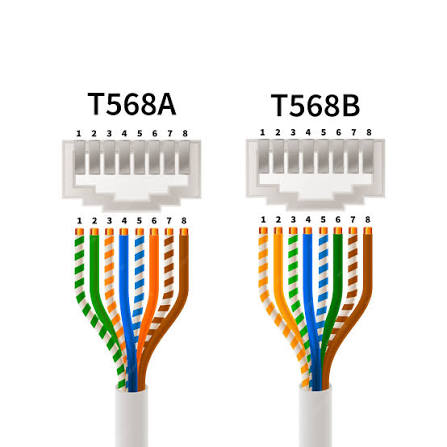
\includegraphics[width=\textwidth]{assets/fotos_cable_utp/foto1_colores.jpg}
    \caption{Paso 5 -- Orden de colores T568B}
  \end{subfigure}
  \hfill
  \begin{subfigure}[t]{0.47\textwidth}
    \centering
    \fbox{\parbox{0.9\textwidth}{\centering\vspace{2.5cm}\small\itshape\color{gray}
      IMAGEN REQUERIDA\\[4pt]
      Subir: \texttt{assets/fotos\_cable\_utp/}\\
      \texttt{foto2\_crimpado.jpg}\\[4pt]
      (Conector RJ-45 Cat 6 en crimpadora)
      \vspace{2.5cm}}}
    %% 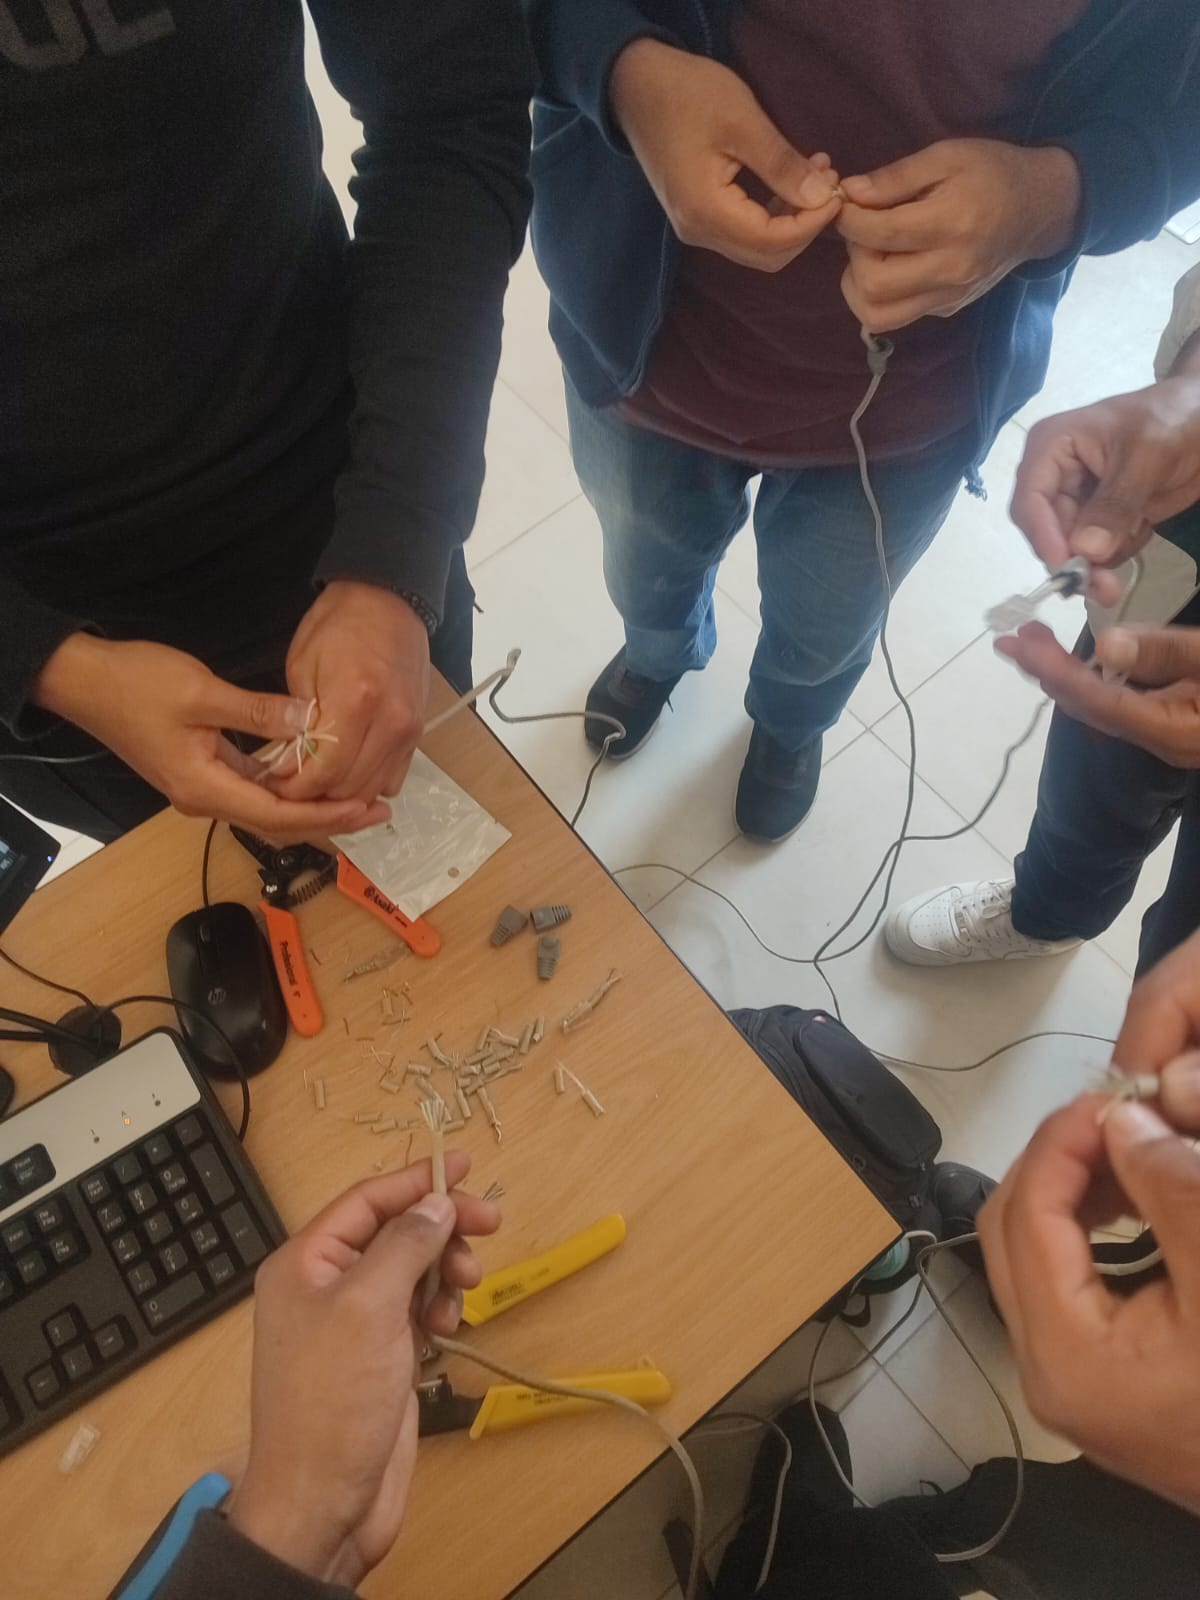
\includegraphics[width=\textwidth]{assets/fotos_cable_utp/foto2_crimpado.jpg}
    \caption{Paso 8 -- Crimpado con tenaza}
  \end{subfigure}
  \vspace{10pt}
  \begin{subfigure}[t]{0.47\textwidth}
    \centering
    \fbox{\parbox{0.9\textwidth}{\centering\vspace{2.5cm}\small\itshape\color{gray}
      IMAGEN REQUERIDA\\[4pt]
      Subir: \texttt{assets/fotos\_cable\_utp/}\\
      \texttt{foto3\_cable.jpg}\\[4pt]
      (Cable terminado con capuchones)
      \vspace{2.5cm}}}
    %% 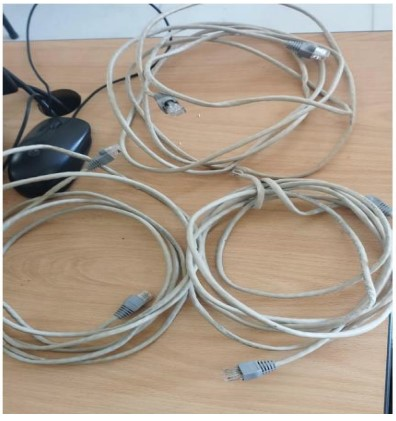
\includegraphics[width=\textwidth]{assets/fotos_cable_utp/foto3_cable.jpg}
    \caption{Cable UTP terminado -- T568B}
  \end{subfigure}
  \hfill
  \begin{subfigure}[t]{0.47\textwidth}
    \centering
    \fbox{\parbox{0.9\textwidth}{\centering\vspace{2.5cm}\small\itshape\color{gray}
      IMAGEN REQUERIDA\\[4pt]
      Subir: \texttt{assets/fotos\_cable\_utp/}\\
      \texttt{foto4\_tester.jpg}\\[4pt]
      (LAN Tester con 8 LEDs secuenciales)
      \vspace{2.5cm}}}
    %% \includegraphics[width=\textwidth]{assets/fotos_cable_utp/foto4_tester.jpg}
    \caption{LAN Tester -- 8 LEDs secuenciales OK}
  \end{subfigure}
  \caption{Registro fotografico del cable UTP Cat 6 construido por el equipo (T568B)}
\end{figure}

\subsection{Anexo D: Plano Arquitectonico de la Biblioteca (Miro / Draw.io)}

%% ┌────────────────────────────────────────────────────────────────────────────┐
%% │ IMAGEN REQUERIDA -- Exportar el plano de Miro/Draw.io como PNG y colocar: │
%% │   assets/plano/plano_biblioteca_final.png                                  │
%% │ Luego descomentar el \includegraphics y eliminar el \fbox                  │
%% └────────────────────────────────────────────────────────────────────────────┘

\begin{figure}[H]
  \centering
  \fbox{\parbox{0.9\textwidth}{\centering\vspace{3cm}\small\itshape\color{gray}
    IMAGEN REQUERIDA: Plano Arquitectonico Completo de la Biblioteca\\[8pt]
    Subir al repositorio como: \texttt{assets/plano/plano\_biblioteca\_final.png}\\[6pt]
    Exportar desde Miro o Draw.io en alta resolucion (min.\ 2000 px de ancho)\\[6pt]
    Debe mostrar: distribucion de ambientes, ubicacion de Wall Mounts,\\
    APs en techo, Ceiling Mount, rutas de canaletas y etiquetas de dispositivos.
    \vspace{3cm}}}
  %% \includegraphics[width=\textwidth]{assets/plano/plano_biblioteca_final.png}
  \caption{Plano arquitectonico con ubicacion de dispositivos y rutas de canalizacion -- Biblioteca ``La Cantera''}
\end{figure}

\vspace{16pt}

\noindent\colorbox{azulUni}{\parbox{\textwidth}{\centering\vspace{0.35cm}
  {\small\color{white}
    \textbf{Fin de la Memoria Tecnica de Ingenieria} \quad|\quad
    Redes de Comunicacion I -- Unidad I \quad|\quad
    Biblioteca ``La Cantera'' \quad|\quad
    Octubre, 2026}
  \vspace{0.35cm}}}

\end{document}

